%% This is a tikz file

% This file is set up to use 11pt palatino font.
\tikzset{node lower left/.style={font=\scriptsize,anchor=north east,yshift=-0.032cm,text height=0.198cm,text depth=0.079cm,inner sep=0.03cm},
leaf/.style={font=\normalsize,anchor=west,text height=0.271cm,text depth=0.109cm,inner sep=0.13cm},
node upper left/.style={font=\scriptsize,anchor=south east,yshift=-0.032cm,text height=0.198cm,text depth=0.079cm,inner sep=0.03cm},
bracket label/.style={font=\normalsize,anchor=west,text height=0.271cm,text depth=0.109cm,inner sep=0.2cm},
node upper right/.style={font=\scriptsize,anchor=south west,text height=0.198cm,text depth=0.079cm,inner sep=0.03cm},
node right/.style={font=\scriptsize,anchor=west,text height=0.198cm,text depth=0.079cm,inner sep=0.03cm},
branch/.style={font=\tiny,text height=0.149cm,text depth=0.059cm,inner sep=0.025cm},
root/.style={font=\normalsize,anchor=east,text height=0.271cm,text depth=0.109cm},
node lower right/.style={font=\scriptsize,anchor=north west,text height=0.198cm,text depth=0.079cm,inner sep=0.03cm}}
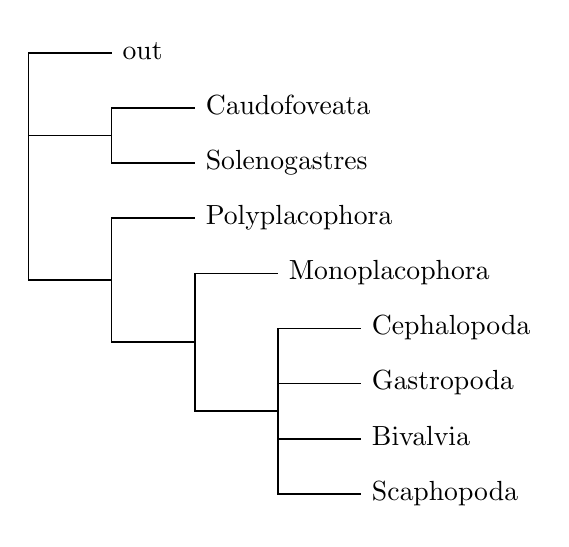
\begin{tikzpicture}[semithick,inner sep=0.1cm]
% +---------1:out
% |
% |         +---------3:Caudofoveata
% |---------2
% 0         +---------4:Solenogastres
% |
% |         +---------6:Polyplacophora
% |         |
% +---------5         +---------8:Monoplacophora
%           |         |
%           +---------7         +---------10:Cephalopoda
%                     |         |
%                     |         |---------11:Gastropoda
%                     +---------9
%                               |---------12:Bivalvia
%                               |
%                               +---------13:Scaphopoda

% The scale is 10.552500, and the yScale is 0.700000

%% Coordinates of nodes.
\coordinate (n0) at (0.000,4.156);
\coordinate (n1) at (1.055,5.600);
\coordinate (n1p) at (0.000,5.600);
\coordinate (n2) at (1.055,4.550);
\coordinate (n2p) at (0.000,4.550);
\coordinate (n3) at (2.111,4.900);
\coordinate (n3p) at (1.055,4.900);
\coordinate (n4) at (2.111,4.200);
\coordinate (n4p) at (1.055,4.200);
\coordinate (n5) at (1.055,2.712);
\coordinate (n5p) at (0.000,2.712);
\coordinate (n6) at (2.111,3.500);
\coordinate (n6p) at (1.055,3.500);
\coordinate (n7) at (2.111,1.925);
\coordinate (n7p) at (1.055,1.925);
\coordinate (n8) at (3.166,2.800);
\coordinate (n8p) at (2.111,2.800);
\coordinate (n9) at (3.166,1.050);
\coordinate (n9p) at (2.111,1.050);
\coordinate (n10) at (4.221,2.100);
\coordinate (n10p) at (3.166,2.100);
\coordinate (n11) at (4.221,1.400);
\coordinate (n11p) at (3.166,1.400);
\coordinate (n12) at (4.221,0.700);
\coordinate (n12p) at (3.166,0.700);
\coordinate (n13) at (4.221,0.000);
\coordinate (n13p) at (3.166,0.000);

%% horizontal lines
\draw (n1p) -- (n1);
\draw (n2p) -- (n2);
\draw (n3p) -- (n3);
\draw (n4p) -- (n4);
\draw (n5p) -- (n5);
\draw (n6p) -- (n6);
\draw (n7p) -- (n7);
\draw (n8p) -- (n8);
\draw (n9p) -- (n9);
\draw (n10p) -- (n10);
\draw (n11p) -- (n11);
\draw (n12p) -- (n12);
\draw (n13p) -- (n13);

%% vertical lines
\draw [line cap=rect] (n1p) -- (n5p);
\draw [line cap=rect] (n3p) -- (n4p);
\draw [line cap=rect] (n6p) -- (n7p);
\draw [line cap=rect] (n8p) -- (n9p);
\draw [line cap=rect] (n10p) -- (n13p);

%% leaf labels
\node [leaf,text height=0.271cm,text depth=0.109cm] at (n1) {out};
\node [leaf,text height=0.271cm,text depth=0.109cm] at (n3) {Caudofoveata};
\node [leaf,text height=0.271cm,text depth=0.109cm] at (n4) {Solenogastres};
\node [leaf,text height=0.271cm,text depth=0.109cm] at (n6) {Polyplacophora};
\node [leaf,text height=0.271cm,text depth=0.109cm] at (n8) {Monoplacophora};
\node [leaf,text height=0.271cm,text depth=0.109cm] at (n10) {Cephalopoda};
\node [leaf,text height=0.271cm,text depth=0.109cm] at (n11) {Gastropoda};
\node [leaf,text height=0.271cm,text depth=0.109cm] at (n12) {Bivalvia};
\node [leaf,text height=0.271cm,text depth=0.109cm] at (n13) {Scaphopoda};

\end{tikzpicture}
